%# -*- coding: utf-8-unix -*-
%%==================================================
%% chapter01.tex for SJTU Master Thesis
%%==================================================

%\bibliographystyle{sjtu2}%[此处用于每章都生产参考文献]
\chapter{主要理论与方法}
\label{chap:theory}

\section{期权定价理论}

期权,顾名思义,"期"代表了未来的一个时刻,“权”代表了一种权利。因此,期权即是代表了持有人在未来拥有的某一种收益权利的凭证。期权又作为一种衍生产品,其价值并非凭空产生,而是会依赖于某一种标的资产的价格或价格变动路径。根据这一依赖关系分类,最为简单的期权是欧式期权,其行使权利的时间点确定,并且到期时期权的价值只取决于到期当天标的资产的价格。其他以此关系分类的期权如美式期权,它的价值的确定的规则与欧式期权类似,但是可以在到期日之前提前行权,即在到期日之前根据当日标的价格确定期权价值,以此行使权利;亚式期权,它的价值不像欧式期权或美式期权那样取决于某日的标的价格,而是取决于一些交易日价格的均值,根据这一均值计算方法的不同,又分为几何平均亚式期权和算术平均亚式期权。除此之外,还有很多奇异期权(exotic option),如二项期权、鲨鱼鳍期权、敲入-敲出期权等,它们行权时间各异,对标的价格的依赖关系更为复杂,有些甚至依赖于不止一种标的资产的价格。虽然期权种类有很多,然而,正如塔勒布\cite{taleb1997dynamic}在《动态对冲(Dynamic Hedging)》中所说,由于对复杂的期权的监控和复制非常困难,因此长期来看,市场需求总是会趋向于简单的资产。因此,目前交易量最大的、开仓量最多的,仍是美式期权和欧式期权等较为简单的期权。本文之后讨论将以欧式期权为主。

根据行使的权利的种类不同,欧式期权又可以分为看涨期权和看跌期权。所有的欧式期权都会伴随有一个行权价,看涨期权是指持有人在到期日当天可以以行权价买入标的资产,看跌期权是指持有人在到期日当天可以以行权价卖出标的资产。期权的“权利”特点的体现在持有人的选择权上。当价格有利时,如在看涨期权的到期日标的资产的价格高于行权价,持有人可以选择行使期权,获得这一部分差价带来的收益;相反,当价格不利时,持有人可以可以放弃行权,在当天也不会有任何损失。期权的这一“选择权”的特性也即意味着它不同于期货合约,由于未来期权的持有人可能获得的收益将始终大于或等于0,因此期权持有人需要为这一选择权支付一定的价格,如何确定期权的价格成为了早期金融学研究中诸多学者讨论的话题。同时,由于期权的收益在价格上涨和下跌两个方向上并不对称,这一非对称性意味着期权是一种非线性的资产,期权的非线性的性质也为其定价增加了难度。

1973年,Black和Scholes\cite{black1973pricing}在前人研究的基础之上,提出了Black-Scholes期权定价模型(BS模型),这一模型成为了第一个可应用于实际生产中的的期权定价模型。他们首先设计一个包含期权和标的资产的、完全对冲了价格变动的方向性风险的组合。基于无套利原则,这一组合在一个较短时间间隔内应只获得无风险收益。根据这一等式关系构造了Black-Scholes方程,之后,再通过欧式期权到期日的收益结构,设置边值条件,进而求解得出BS模型。BS模型的提出是划时代的,它不仅解决了欧式期权定价这一问题,直接促进了芝加哥期权交易所的诞生和之后期权交易的飞速增长\cite{mackenzie2008engine},更重要的是,它的推导过程及背后的思想提供了期权定价的一个基本范式,为之后各类期权及其他衍生产品的定价奠定了基础。

BS模型是建立在一系列严格的假设之上的,这些假设包括:

\begin{enumerate}
    \item 标的资产的对数收益率服从几何布朗运动,即$dS/S=\mu dt+\sigma dW$。
    \item 卖空所得可以全部用于在投资且无需考虑保证金问题。
    \item 标的资产可以无限分割且交易时无交易费用。
    \item 标的资产不会产生收益(比如股利)。
    \item 市场中不存在无风险套利机会。
    \item 标的资产的交易是连续的。
    \item 无风险利率r是常数且适用于所有期限资金的借贷。
\end{enumerate}

基于以上假设,可以得出欧式看涨期权价格C为
\begin{equation}
  C=N(d_1)S_t-N(d_2)Ke^{-rT}
\end{equation}
欧式看跌期权价格P为
\begin{equation}
  P=N(-d_2)Ke^{-rT}-N(-d_1)S_t
\end{equation}
其中,
\begin{equation}
  d_1=\frac{1}{\sigma \sqrt{T}}[ln(\frac{S_t}{K}+(r+\frac{\sigma ^2}{2})T)]
\end{equation}
\begin{equation}
  d_2=d_1-\sigma \sqrt{T}
\end{equation}

在上述公式中,

\begin{itemize}
  \item $N(\cdot)$为标准正态分布的累计概率密度函数
  \item $T$为到期剩余时间
  \item $S_t$为标的资产的价格
  \item $K$为行权价
  \item $r$为年化无风险利率
  \item $\sigma$为标的资产的年化标准差
\end{itemize}

虽然经典的期权定价模型依赖于诸多假设,有些假设甚至和现实情况差异较大,但是,由于其表达简单直观,计算迅速,因此,这一模型在实际生产中应用较多。本文仍将根据这一模型进行模拟研究和实证研究中,之后在此基础之上再进行扩展的讨论。

\section{希腊字母}

从期权定价公式中,可以看出期权的价格取决于诸多变量,包括行权价格、标的资产价格、标的资产波动率、到期剩余时间和无风险利率。根据BS模型的假设,在这些变量中,实际上只有标的资产价格是随机的,其他变量都是可以事先确定的。因此,在模拟研究的动态对冲中,我们较为关心期权价格如何随标的资产价格的变化而变化,也就是期权价格对标的资产价格的敏感性。衡量这一敏感性的指标为希腊字母。本节将详细介绍和标的资产价格有关的希腊字母及其在动态对冲中的应用,同时也会简要介绍其他常用的希腊字母以及希腊字母之间的某些联系。

\subsection{Delta}

在BS模型的推导中,Black和Scholes构造了一个对冲组合,这一对冲组合的价值在瞬时是不受标的资产价格变动的影响的。该对冲组合的构建即使用到了希腊字母——Delta($\Delta$)。Delta衡量的是标的资产价格S变动时,期权价格V变动的幅度,即V对S的一阶导数,其计算方式为
\begin{equation}
  \Delta=\frac{\partial V}{\partial S}
\end{equation}
根据上一节的BS模型,可以计算得出看涨期权的Delta值为
\begin{equation}
  \Delta=N(d_1)
\end{equation}
看跌期权的Delta值为
\begin{equation}
  \Delta=N(d_1)-1
\end{equation}

Delta值的计算是动态对冲的关键。动态对冲中的对冲组合的具体构造方法如下:起始时刻卖出一份期权同时持有Delta份标的资产,之后在每个再平衡(rebalance)时刻,调整组合中标的资产,使其数量等于该时刻持有的期权的Delta值。因此,在动态对冲中,决定性的因素有两个:1)再平衡时刻的Delta值。2)再平衡时刻的选取。关于这两个因素的确定及其影响因素,我们将在之后予以介绍。

\begin{figure}[htb]
  \centering
  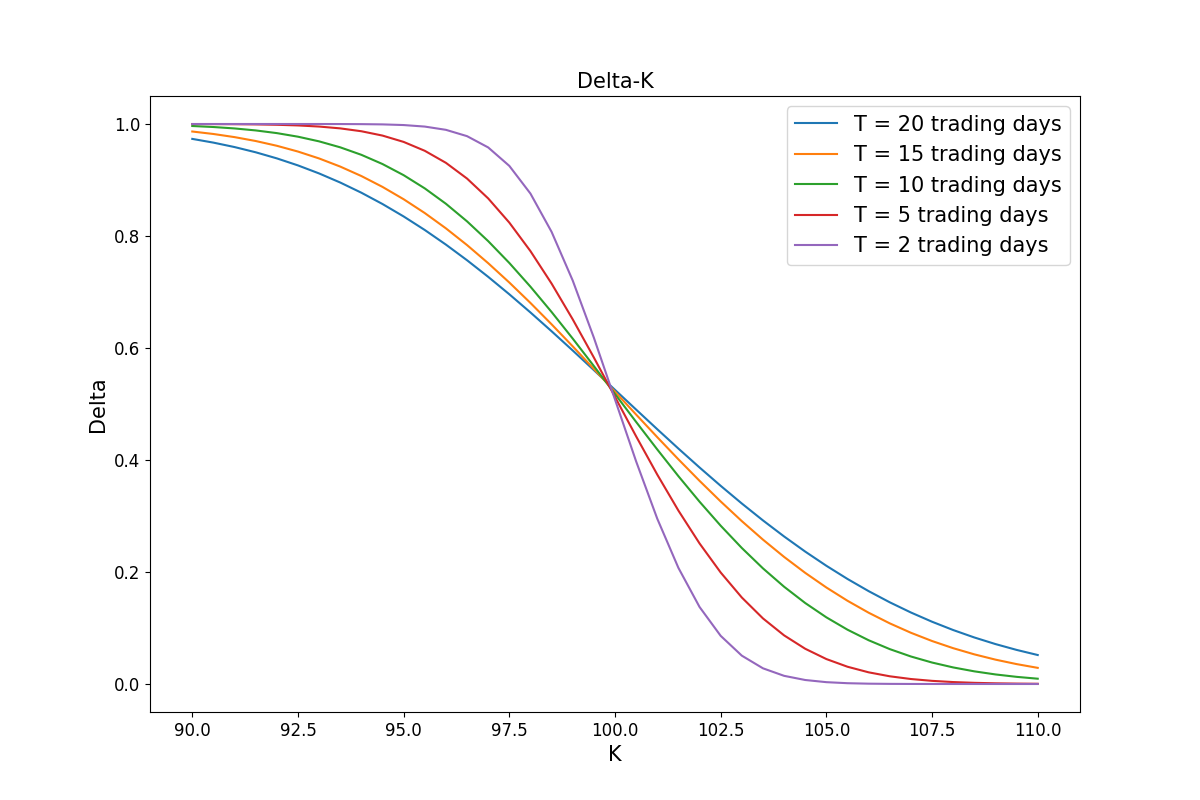
\includegraphics[width=10.8cm, height=7.2cm]{theory/delta_K.png}
  \caption[这里将出现在插图索引中]
    {看涨期权Delta与K和T的关系}
  \label{fig:delta_k}
\end{figure}

\begin{figure}[htb]
  \centering
  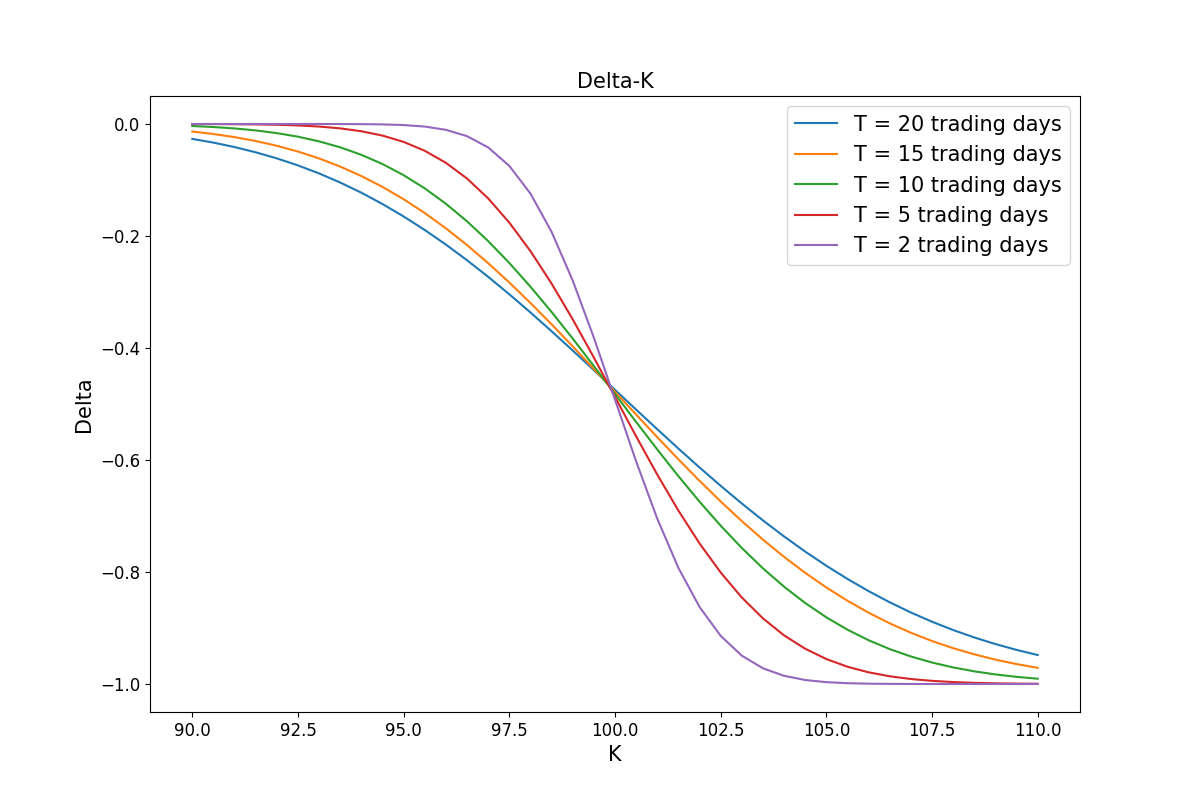
\includegraphics[width=10.8cm, height=7.2cm]{theory/put_delta_K.png}
  \caption[这里将出现在插图索引中]
    {看跌期权Delta与K和T的关系}
  \label{fig:put_delta_k}
\end{figure}

看涨期权和看跌期权的Delta与行权价K和到期剩余时间T的关系分别如图\ref{fig:delta_k}和图\ref{fig:put_delta_k}所示。对于看涨期权来说,Delta始终为正,并且行权价K越高,Delta的绝对值越低;对于看跌期权来说,Delta始终为负,并且行权价K越高,Delta的绝对值越高,这其实可以从Delta的性质得到直观的理解。以看涨期权为例,Delta的计算公式为$N(d_1)$,这一值与$N(d_2)$的值非常接近,并且两者的差值与K无关。而$N(d_2)$代表了在风险中性世界里,到期日标的价格达到K以上的概率,即看涨期权在到期日被行权的概率。因此,行权价K越高,看涨期权在到期日被行权的概率越低,Delta的绝对值越低;看跌期权与其同理。同时,无论是看涨期权还是看跌期权,Delta的绝对值均在0到1之间,并且随着到期日的临近,虚值期权的Delta的绝对值逐渐趋近于0,实值期权的Delta的绝对值逐渐趋近于1。这也可以很直观地从Delta的性质中得到解释:随着到期日临近,留给虚值期权进入实值和实值期权进入虚值的机会都越来越小,因此,它们的Delta的绝对值分别向0和1收敛。

\subsection{Gamma}

在动态对冲中,Delta是我们需要主要关注的对象。但是,由于期权是一种非线性资产,它的Delta值会随着标的资产价格的变化而变化。因此,除了Delta本身的大小之外,我们还需要关注Delta对标的资产价格变化的敏感性。衡量这一敏感性的希腊字母即为Gamma。Gamma是期权价格V对标的资产价格S的二阶导数,其计算方式如下:
\begin{equation}
  \Gamma=\frac{\partial^2 V}{\partial S^2}
\end{equation}
由此得出看涨期权的Gamma和看跌期权Gamma的表达式相同,均为
\begin{equation}
  \Gamma=\frac{N'(d_1)}{S\sigma\sqrt(T)}
\end{equation}

对于看涨期权和看跌期权,Gamma始终为正。Gamma绝对值的大小影响了动态对冲组合再平衡的频率,即前文所说的动态对冲的第二个决定因素。当Gamma的绝对值较小时,Delta受标的资产价格变动的影响较小,对冲者若有一定的风险承受能力,选择可以暴露较小的Delta,就不需要频繁地调整组合的Delta,即使需要调整每次调整的幅度也不会很大;相反,如果Gamma的绝对值较大时,则相对较小的标的资产价格的变动也会带来组合Delta的很大的变动,此时对冲者就需要更频繁地、更大幅度地调整组合的Delta值,以使组合Delta的暴露回到风险承受范围之内。对于期权策略组合来说,可以通过买卖期权来实现Gamma中性。然而,对于动态对冲组合,由于只能使用线性工具进行对冲,对冲者并不能改变组合的Gamma。因此,在动态对冲中,通过确定再平衡时点以及在再平衡时点买卖线性工具,与其说是对Delta这一一次风险进行对冲,不如说是使用线性工具来逼近一个二次函数,即是对Gamma风险进行管理。

\begin{figure}[htb]
  \centering
  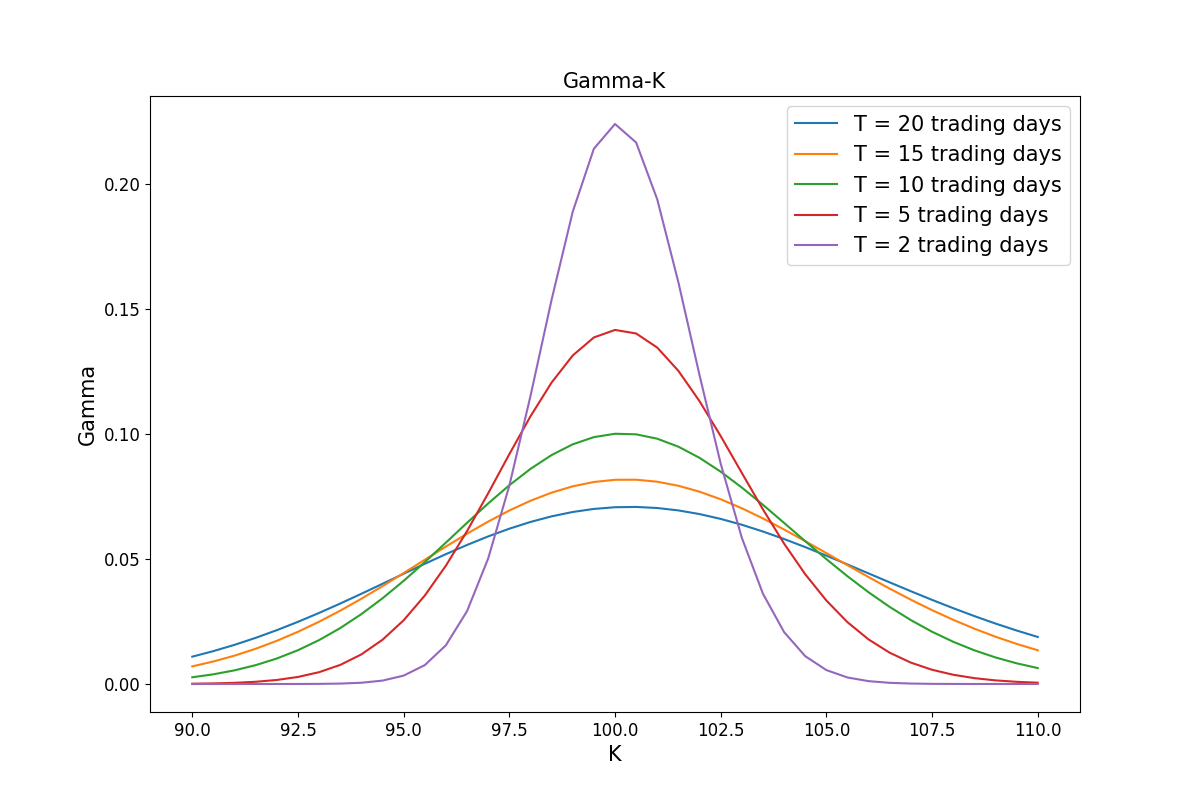
\includegraphics[width=12cm, height=8cm]{theory/gamma_K.png}
  \caption[这里将出现在插图索引中]
    {Gamma与K和T的关系}
  \label{fig:gamma_k}
\end{figure}

Gamma与行权价K和到期剩余时间T的关系如图\ref{fig:gamma_k}所示。无论看涨期权还是看跌期权,平值附近的Gamma最高。并且随着到期日的临近,平值期权的Gamma逐渐增大且Gamma对K的分布越来越呈现出“尖峰”的特点。因此,一般而言,到期剩余时间越短,再平衡频率需要增高以更好地管理Gamma风险。到期当日时,由于平值附近的期权往往会游离于实值和虚值之间,其Delta的绝对值则在1和0之间变化,Gamma也会非常高。这时的Gamma风险又被称为大头针风险(pin risk)。对于一般的期权交易者来说,最好的管理大头针风险的方式就是提前展期,不持有临近到期的期权;然而,对于场外期权交易商而言,在动态对冲中他们必须要面对这一风险,如何更好地管理大头针风险也是场外期权交易商面临的一个难题。

\begin{figure}[htb]
  \centering
  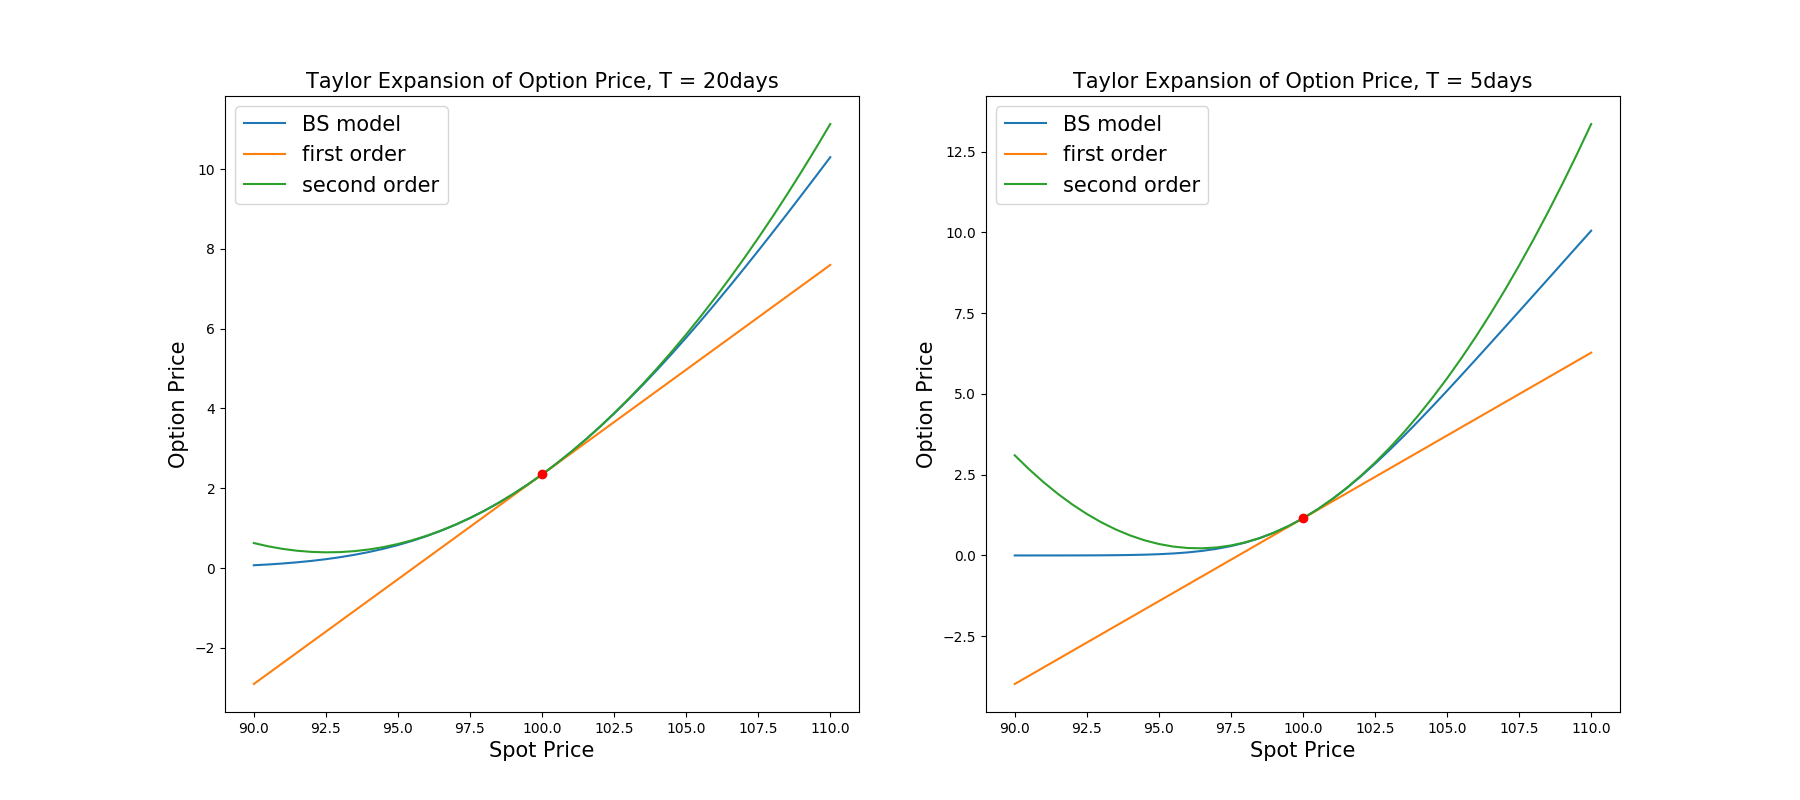
\includegraphics[width=16cm, height=7cm]{theory/taylor.png}
  \caption[这里将出现在插图索引中]
    {平值看涨期权价格的泰勒展开}
  \label{fig:taylor}
\end{figure}

至于使用Gamma可以从多大精度上拟合标的价格,可以参见图\ref{fig:taylor}。该图分别展示了到期剩余时间为20日和5日时,平值看涨期权价格随标的价格的变化情况,定价时使用的年化波动率为20\%。从图中可以看出,在到期时间剩余20日时,使用二次函数在标的价格上下约5\%的范围内可以较好地拟合BS模型的价格;随着到期日的逐渐临近,在到期时间剩余5日时,使用二次函数只能在标的价格上下约2\%的范围内较好地拟合BS模型的价格。这与到期日临近时,Gamma逐渐呈现“尖峰”的特点有关。

\subsection{其他希腊字母}

除了Delta和Gamma这两个和标的资产价格相关的希腊字母之外,常用的希腊字母还有Theta、Vega和Rho,本小节将一一予以介绍。

\subsubsection{Theta}

Theta是指期权价格对时间变化的敏感性,即期权价格V对到期剩余时间T的一阶导数。一般来说,对于看涨期权和看跌期权,Theta始终为负。在其他条件不变的情况下,到期剩余时间是始终递减的,期权价格在Theta上的变化是可以确定的,因此Theta又被称为期权的时间价值。对于需要动态对冲的场外期权空头方而言,在进行了Delta的对冲之后,对冲组合有正的Theta,看起来可以获取一个稳定的时间价值。实际上,这也是很多期权卖方策略中收益的主要来源。

然而,在考虑时间价值时,不能够单独考虑Theta,而是要把Gamma一起纳入考量。对于场外期权空头方,他们之所以有一个始终为正的Theta暴露来收取一个看似稳定的时间价值,是因为他们同时有负的Gamma暴露。随着每天时间的流逝,只要标的资产的价格有所波动,空头方在Gamma上总会有一定的损失。与Theta稳定的收益不同的是,Gamma上的损失的大小取决于当日标的资产价格波动的绝对值的大小。因此,正的Theta是对暴露的Gamma风险的补偿。当然,Theta上的收益并不是总能够补偿Gamma上的损失的。BS方程实际上就定量地反映了这一补偿关系。根据BS方程
\begin{equation}
  (-\frac{\partial V}{\partial t} - \frac{1}{2}\sigma^2S^2\frac{\partial^2 V}{\partial S^2})\Delta t=r(-V+S\frac{\partial V}{\partial S})\Delta t
\end{equation}
等式右边表明完全对冲掉Delta的对冲组合在$\Delta t$时间内只能够获得无风险收益。将等式左边改写,使用希腊字母替代偏导数
\begin{equation}
  -\Theta \Delta t - \frac{1}{2}\Gamma(\sigma \sqrt{\Delta t} S)^2=r(-V+S\frac{\partial V}{\partial S})\Delta t
  \label{eq:bs}
\end{equation}

式\ref{eq:bs}左边第一项代表了在$\Delta t$时间内,场外期权空头方在Theta上的收益,第二项代表了场外期权空头方在Gamma上的损失。注意此处的$\sigma$是在期权定价模型中使用的波动率。因此,从直观上理解,可以认为$\sigma \sqrt{\Delta t}$代表了维持Theta的收益和Gamma的损失等于无风险收益时,标的资产实际变化率的绝对值。当标的资产的实际变化率等于该值时,对冲组合在$\Delta t$时间内只能获得无风险收益;当标的资产的实际变化率大于该值时,对冲组合将获得小于无风险收益的收益;当标的资产的实际变化率小于该值时,对冲组合将获得大于无风险收益的收益。这一等式揭示了场外期权空头方的收益和风险来源,对场外期权定价以及动态对冲实际操作中的风险控制有着重要意义。关于该式的更详细的讨论,将在下一节中进行。

\subsubsection{Vega}

Vega是指期权价格对标的资产波动率的敏感性,一般是一个正数。在动态对冲中,如果整个过程使用固定的波动率,则Vega不会成为损益的来源,其主要的应用是在场内期权的交易中。由于场内期权的波动率不断变化,因此场内期权交易者不能忽视在Vega上的损益,有时Vega上的损益甚至会占到策略损益的主要部分。关于Vega的更进一步的讨论将在下一节进行。

\subsubsection{Rho}

Rho是指期权价格对无风险利率的敏感性。一般情况下,当标的波动率相对于无风险利率较大时,Rho并不成为我们在动态对冲中考虑的因素。对于某些特定的标的,如外汇,其波动率较小(年化波动率一般在10\%以下),此时Rho会显得更为重要。

\section{波动率}

BS模型假设标的资产的收益率服从几何布朗运动,其波动率是一个事先确定的常数。然而,在实际市场中,首先我们无法确定标的资产波动率是否是一个常数,其次我们也无法直接先验地得到这一波动率。同时,在实际生产的期权定价中,如果以当前时点做决策,行权价格、标的资产价格、到期剩余时间和无风险利率都是已知量,需要决定的是定价时采用的标的资产波动率的值。也就是说,在做期权定价时,标的资产波动率和其他变量不同,是需要我们通过某种方式来估计而非可以直接确定的。本节将对期权定价模型中和动态对冲中所使用的波动率进行简要介绍,之后将介绍在实证研究的动态对冲中确定标的资产波动率的几种方法。

\subsection{隐含波动率}

隐含波动率是期权实际交易中的常用指标。在对期权的定价中,一般我们需要事先估计波动率,之后使用定价模型进行定价。对于场内期权而言,其价格由市场参与者通过买卖行为而非使用某种定价模型来确定,此时期权的价格是已知的。由于标的资产波动率和期权价格之间存在着一一对应的关系,并且期权定价中所使用的其他变量都是已知的,因此可以使用数值的方法,如牛顿法、二分法等计算出期权价格对应的波动率。这一波动率又被称为隐含波动率。

期权定价模型中的波动率是标的资产未来的波动率,因此隐含波动率代表了市场对标的资产未来的波动率大小的估计。准确来说,隐含波动率代表的是标的资产从当天到到期日的年化波动率大小。隐含波动率越大,代表标的资产未来的波动率越大。由于期权到期日的收益是不对称的,标的资产未来的波动率越大,期权越有可能进入实值状态,其到期日收益的期望越大。因此隐含波动率越大,期权价格越高。这也说明了为什么Vega始终为正。

\begin{figure}[htb]
  \centering
  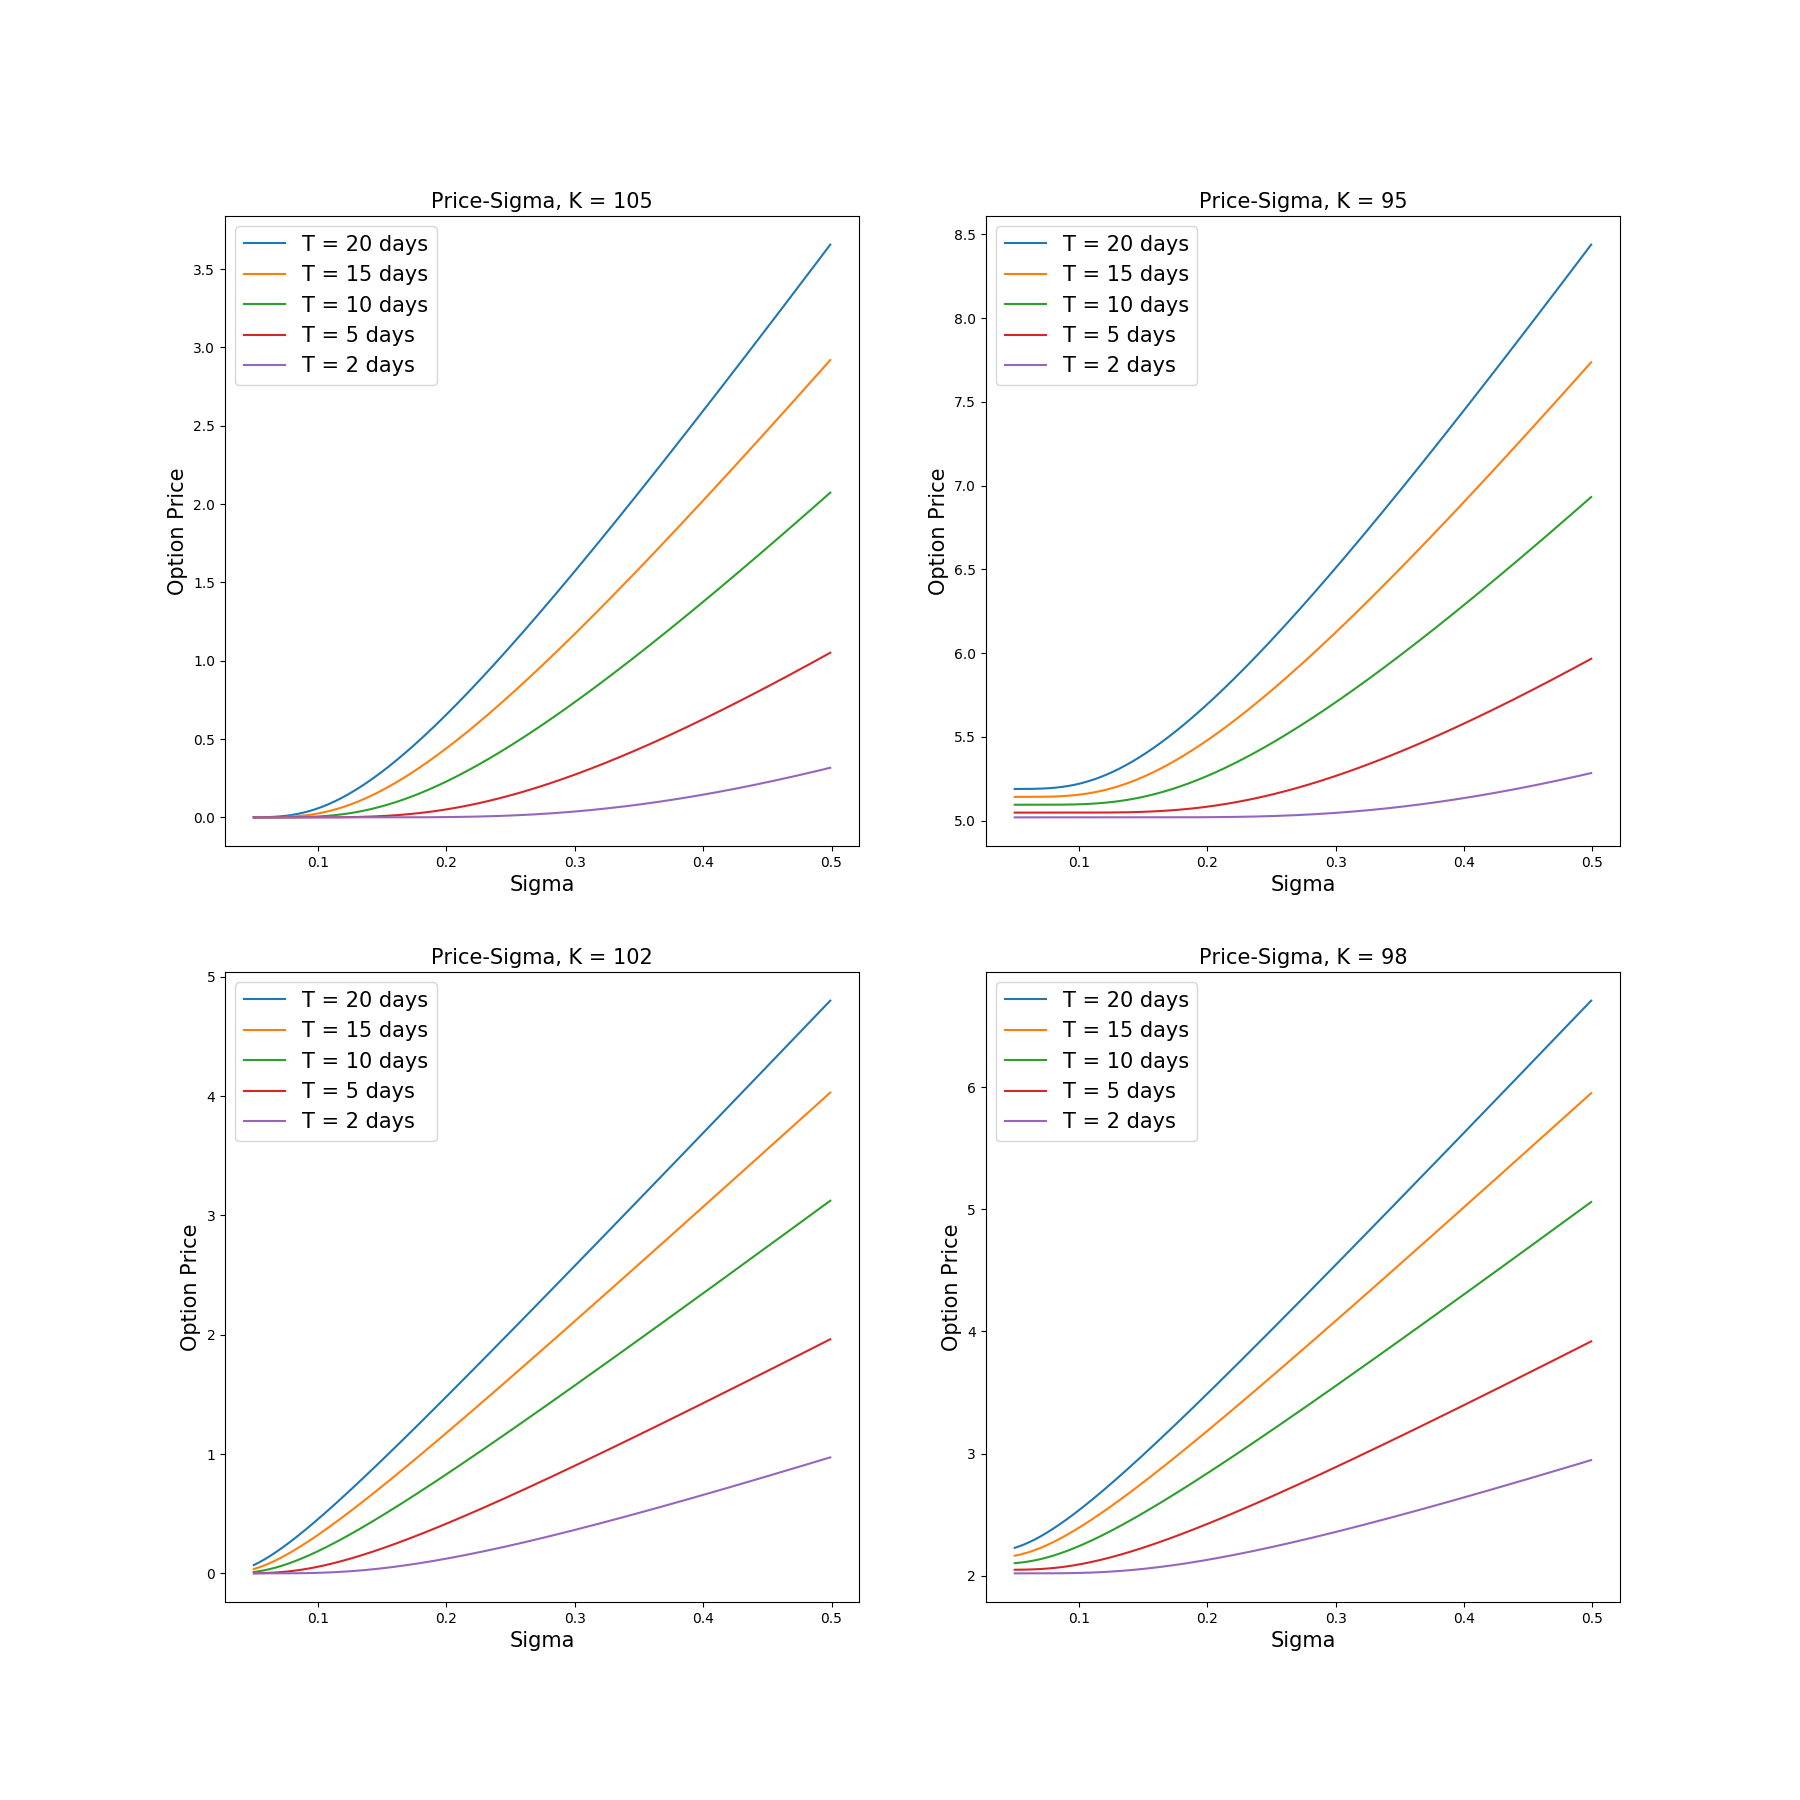
\includegraphics[width=16cm, height=16cm]{theory/sigma_prc.png}
  \caption[这里将出现在插图索引中]
    {看涨期权价格和隐含波动率}
  \label{fig:sigma_prc}
\end{figure}

图\ref{fig:sigma_prc}展示了不同行权价的期权在不同到期剩余时间下看涨期权的价格和隐含波动率的关系。从图中可以看出,对于虚值和实值的期权,随着到期日的临近,在隐含波动率较小时期权价格对隐含波动率变得越来越不敏感,并且这一不敏感的区间逐渐扩大。例如行权价为105的看涨期权,在到期剩余时间为2个交易日时,隐含波动率在大约30\%之内变化对其价格都影响不大。这是因为到期剩余时间较小,虚值程度较深,因此在仅有的2个交易日内标的资产必须要有非常大的波动,该期权才有可能进入实值,否则到期时价值将归零。这也说明随着到期日的临近,Vega对行权价K的分布也会越来越展现出“尖峰”的特点。

隐含波动率的确定在场外期权的动态对冲中有着重要的意义,隐含波动率的大小决定了动态对冲组合在未来所获得的期望收益的大小。具体而言,隐含波动率对于场外期权的空头方来说,是属于需要做出决策的变量,确定隐含波动率的大小即确定了卖出的期权的价格。根据式\ref{eq:bs},若未来标的资产的实际波动率高于定价时所用的隐含波动率,则场外期权空头方将会有一个低于无风险收益的期望收益;反之,若标的资产的实际波动率低于定价时的所用的隐含波动率,则场外期权的空头方将会有一个高于无风险收益的期望收益。因此,在确定隐含波动率之前,需要对标的资产未来的实际波动率有一个较为准确的估计,这一估计的准确性将直接影响到最终动态对冲组合的对冲成本大小。

以上是对隐含波动率对动态对冲影响的理论上的直观解释。具体到动态对冲的操作上,我们之前提到动态对冲中有两个需要确定的因素,一个是再平衡时刻的Delta值,另一个是再平衡时刻的选取。在确定了隐含波动率之后,使用这一波动率根据BS模型计算出Delta值,就确定了动态对冲的第一个因素。因此,与其说在每个再平衡时刻需要确定Delta值,不如说需要确定计算Delta值使用的隐含波动率,也就是估计标的资产未来收益率的波动率。实际生产中,我们需要做的,也即是找到一个尽可能准确的方法,来对标的资产未来收益率的波动率做出估计,再以此波动率计算Delta值用于对冲组合的再平衡。

\subsection{实际波动率}

上一小节我们提到,在实际动态对冲中确定未来标的资产的实际波动率是非常关键的,它决定了动态对冲组合每个交易日的期望收益。实际波动率是对一段时间内标的资产价格平均波动幅度的一个估计。在BS模型中使用的波动率为年化波动率,使用历史数据计算年化波动率的方法为收益率的样本方差乘以年化系数
\begin{equation}
  \sigma^2=\tau\sum_{i=1}^n (u_i-\bar{u})^2
\end{equation}
年化系数$\tau$与对数收益率$u$的计算频率有关。设对数收益率$u$对应的时间间隔为$\Delta t$,则$\tau=\frac{1}{\Delta t}$。因此,以日频收益率为例,$\sigma \sqrt{\Delta t}$实际上代表了标的资产的日频波动率。注意到这一日频波动率的计算和上文所说的维持Theta上的收益和Gamma上的损失之和为无风险收益的标的变化率的绝对值相同,这也揭示了式\ref{eq:bs}同实际波动率之间的联系。

对未来的实际波动率的估计方法有很多种,但是大部分方法的基本思想都是认为标的资产的未来的实际波动率将会延续历史规律,因此通过充分挖掘历史信息可以预测未来的实际波动率。由于本文旨在研究动态对冲相关的理论和方法,而未来实际波动率的预测是一个更深层次的问题,本文对这一问题不做详细的探讨,在此仅介绍几种常用的波动率预测方法。

(1)隐含波动率。如果需要定价或对冲的场外期权有对应的场内期权的话,场内期权的隐含波动率是未来实际波动率的一个很好的估计,具体原理在上一小节有所讨论。然而,大多数情况下,场外期权交易商交易的期权一般都没有对应的场内期权或场内期权交易很不活跃。因此,这一方法虽然效果较好,但是实际操作中难以应用。

(2)历史波动率。使用历史波动率作为对未来波动率的预测是最为简单的波动率预测方法。这一方法假设预测期的收益率数据和所用的历史收益率数据有着相同的分布特点,因此可以通过直接计算历史数据的样本标准差来对未来的波动率进行预测。计算简单、速度快是历史波动率方法的优势;然而,由于这一方法过于简单,在预测时会忽略掉历史数据中的一些规律,同时,如何决定所用历史数据的长度也是值得讨论的问题。一般习惯上而言,所采用的历史数据长度和预测期长度相同。

(3)指数加权移动平均(exponentially weighted moving average, EWMA)。EWMA波动率的计算方式为
\begin{equation}
  \sigma_t=\frac{\sum_{i=0}^n \beta^iu_{t-i}^2}{\sum_{i=0}^n \beta^i}
\end{equation}
EWMA方法给予了距离当前时点较近的数据更高的权重,认为越近的数据包含了更多的信息,对未来实际波动率预测的价值越大。这一方法的优势在于不需要依赖过多的历史数据,并且可以动态地反映实际波动率的变化并以此做出预测;然而,它不能反映实际波动率均值回复的特点。有时在计算时,会将收益率减去对应的EWMA均值再进行平方,本文将采用这种做法。对于EWMA公式中$\beta$的确定,本文将采用JP Morgan在Riskmetrics数据库中使用的值0.94。

(4)GARCH(1,1)模型。GARCH(1,1)模型其实和EWMA模型类似,但是加入了一个均值回复项,因此可以反映实际波动率均值回复的特点。其递推表达式如下
\begin{equation}
  \sigma_{t+1}=\alpha_0+\alpha_1u_t^2+\beta \sigma_t
\end{equation}
虽然GARCH模型考虑了波动率分布的更多地特点,但是它也有一些不足之处。GARCH模型要求被预测的序列的波动率有平稳性。然而,实际市场中许多资产收益率序列的波动率水平常常会随市场、政策环境等因素发生较大的改变,这使得GARCH模型的预测效果将会变差甚至无法得出稳定的估计参数。

Poon和Granger(2003)\cite{poon2003forecasting}对各个波动率预测方法的预测能力进行过总结。从总结的结果来看,虽然GARCH族模型看似更为复杂,但是其预测能力并没有明显的优势。在基于历史波动率的方法(包括历史波动率和EWMA波动率)和GARCH族模型的比较中,他们统计了39个研究,其中22个研究显示基于历史波动率的方法优于GARCH族模型,17个研究的结果相反。相比之下,从场内期权数据中计算得出的隐含波动率有着最好的预测效果。18个研究比较了隐含波动率和GARCH族模型的优劣,其中17个认为隐含波动率较GARCH族模型更优。实际上,由于隐含波动率使用了和未来实际波动率更相关的信息(场内期权信息),所以其有最强的预测能力;相比之下,无论是GARCH族模型还是基于历史波动率的方法,使用的都是历史收益率信息,因此两者的预测能力并无太大差别。本文在实证研究中,将主要使用历史波动率和EWMA波动率作为对未来实际波动率的预测。

\section{动态对冲策略}

在上文中,我们对动态对冲的基本思想和影响因素已经有了一定的介绍。本文所说的动态对冲是指Delta上的动态对冲。对于场外期权空头方来说,其实现的基本思想如下:在起始时刻,卖出一份期权同时持有Delta份标的资产做对冲,之后在每个再平衡时刻,调整持有的标的资产,使其数量等于该时刻空头期权的Delta值。同时,对于这一过程中产生的资金缺口或盈余,本文假设可以通过以无风险利率借入或贷出。动态对冲的主要结果是对冲成本,对冲成本的具体计算方式将在下一章介绍。

基于之前的分析,我们认为动态对冲的决定性的因素有两个:1)再平衡时刻的Delta值。2)再平衡时刻的选取。关于再平衡时刻的Delta值的确定,我们已经做出了详细的介绍,认为确定某一时刻空头期权Delta值即为估计该时刻标的资产的未来波动率。对于未来波动率的估计方法,我们在上一节有所涉及。本节我们将主要关注再平衡时刻的选取。关于这一因素,我们将通过考察两种动态对冲策略来进行介绍。

\subsection{固定时点动态对冲}

固定时点动态对冲是指选取固定时间间隔的再平衡时刻进行Delta的对冲操作,在对冲起始时刻即确定了所有的再平衡时间点。理论基础简单、易于控制是这一策略的优势。并且,这也是BS模型的推导中所使用的动态对冲策略。Leland(1985)\cite{leland1985option}在推导有交易成本的期权定价模型时,使用的也正是这一策略。然而,这一方法的缺点在于难以确定再平衡时刻的时间间隔。如果时间间隔过短,虽然可以获得较高精度的对冲效果,但是频繁的对冲会使操作的难度增大;若对冲的时间间隔较长,虽然操作时较为简单,但是对冲效果会相应变差。固定时点动态对冲的更大的缺陷在于,当到期日临近时,Gamma会逐渐增大,Delta的波动也会随之增大。若采用的对冲时间间隔较小,则在初始阶段操作频繁,但是对整个组合的Delta暴露影响不大;若采用的对冲时间间隔较大,则在临近到期日时对冲频率与Delta的波动程度无法匹配,对冲精度随之降低。

\subsection{固定Delta区间动态对冲}

与固定时点动态对冲不同,固定Delta区间动态对冲并不会事先确定再平衡时刻。这一策略的基本思想是,首先设定一个固定的Delta阈值,同时选定一个观察Delta的频率。随着时间的变化,在每个Delta观察时刻,当对冲组合的Delta的绝对值暴露超过该阈值时,则进行对冲操作,调整组合的Delta值为0;若对冲组合的Delta的绝对值暴露小于该阈值,则不进行操作。这一策略实质上是基于了Hodges和Neuberger(1989)\cite{hodges1989optimal}及其后续研究的思想,与在效用理论中风险和收益的权衡类似,使用一个较小的Delta风险暴露来平衡对冲带来的交易成本。该策略的关键点在于Delta阈值的确定,相当于是Delta风险和对冲成本之间的权衡。

本文在模拟分析和实证研究中,将主要使用以上两种动态对冲策略。关于交易成本以及动态对冲策略的参数对对冲效果和对冲成本的影响,我们将在下一章进行具体的讨论。

\section{模拟方法}

在动态对冲研究中,模拟方法主要应用在资产价格路径的模拟上。关于资产价格路径的模拟,常用的有蒙特卡洛(Monte Carlo)方法和拟蒙特卡洛(Quasi-Monte Carlo)方法。蒙特卡洛方法是数值模拟中最为常用的方法,它实际上是这一类模拟方法的总称。本文所说的蒙特卡洛方法是一个相对狭义的概念,是指通过生成随机或伪随机(pseudo-random)序列,模拟一个随机事件的可能情况,进而用频率来估计概率的方法。根据大数定律,若想有效地应用蒙特卡洛方法,需要较多的模拟的次数。在本文的研究中,我们并不直接考察每一次模拟的结果,而是对每一次的结果的一个函数进行求期望的操作,这一期望即为蒙特卡洛积分。设模拟次数为N,根据中心极限定理,蒙特卡洛积分的收敛速度为$O(N^{-\frac{1}{2}})$。蒙特卡洛的优势在于,其收敛速度独立于积分的维数。这一特点也使得其鲁棒性非常强,可以适用于很多高维的问题。然而,这一鲁棒性的代价是相对较慢的收敛速度。若要将误差的标准差大小的小数点向后移一位,需要将模拟次数提升为的100倍。

虽然蒙特卡洛方法鲁棒性较好,但是其对计算时间要求较高,因此本文最初希望可以找到一种收敛速度更快同时又不失鲁棒性的方法。我们考察了拟蒙特卡洛方法。拟蒙特卡洛方法使用低差异序列(low discrepancy sequence)进行模拟,经典的低差异序列包括Halton序列、Sobol序列和Faure序列。差异(discrepancy)是用来形容均匀性(uniformity)的,低差异序列比伪随机序列更接近均匀分布。与蒙特卡洛方法使用线性同余法等方法通过生成伪随机序列来试图模仿随机数的性质不同,低差异序列实际上是确定性的序列,并且其具有一定的自相关性来降低差异。因此拟蒙特卡洛方法只能用在蒙特卡罗积分问题上,使用其进行优化或单纯考察其模拟的结果是无意义的。拟蒙特卡洛模拟的收敛速度是$O((logN)^{d}N^{-1})$,其中d为模拟的维数。从这一收敛速度可以看出,当模拟次数N相对于维数d很大时,可以获得接近$O(N^{-1})$的收敛速度。然而,当d增长时,N需要以指数速度增长,以维持相应的收敛速度。如果N不足够大的话,拟蒙特卡洛模拟的收敛速度会慢于蒙特卡洛模拟的收敛速度。正如Caflisch(1998)\cite{caflisch1998monte}指出的,高维性会很大程度上限制拟蒙特卡洛模拟的有效性。具体到本文的研究上,由于动态对冲是一个路径依赖的问题,因此其对应的维数即为标的资产价格路径模拟的频数,这一维数通常会很高(大于50)。在这样高维的模拟下,拟蒙特卡洛模拟效果将不如蒙特卡洛模拟。因此,在之后的研究中,本文将使用蒙特卡洛模拟生成资产价格序列。

当然,蒙特卡洛模拟可以通过方差减少技术来加快收敛速度,这一速度上的提高通常是通过减小$O(N^{-\frac{1}{2}})$项的系数,而并不会将速度提升一个量级,因此,对于这一技术,本文将不深入进行讨论,亦不会在应用中有所体现。关于拟蒙特卡洛模拟在高维情况下表现较差的问题,Wang和Sloan(2008)\cite{wang2008low}给出了一个解决方法,他们使用了一个新的计算差异的算法,使得拟蒙特卡洛方法在高维时的表现优于或至少不弱于蒙特卡洛方法。对于这一算法的细节、实现及应用,本文亦不进行讨论,而是将其作为未来可能的改进方向。

在确定了模拟使用的方法后,我们只是得到了生成参数为$(0,1)$的均匀分布的随机数的方式。获得了这一随机数后,可以使用正态分布的逆变换获得正态分布的随机数。之后,基于标的资产符合几何布朗运动的假设,生成价格序列。在之后的模拟研究中,我们在BS模型的假设之上,改变或增加如下设定:

\begin{itemize}
  \item 买卖标的资产时,交易费用与交易额成比例。
  \item 所有的日期和年化波动率均使用交易日计算,每年252天。
\end{itemize}

\section{本章小结}

本章主要介绍了期权定价和动态对冲的相关理论,重点考察了期权定价和动态对冲之间的联系以及动态对冲的影响因素,对动态对冲的原理和实践进行了剖析,包括未来波动率的估计和动态对冲策略实现方法。同时,也对本文使用的模拟方法和假设进行了简要介绍。
